%
% Átila Camurça <camurca.home@gmail.com>, 2012
%
\section{Introdução}

\begin{frame}

\slidetitle{Introdução}

\end{frame}

\subsection{Ubuntu COMSOLiD 5}

\begin{frame}

\slidesubtitle{Ubuntu COMSOLiD 5}

\end{frame}

\begin{frame}\frametitle{Ubuntu COMSOLiD 5}\framesubtitle{Introdução}

O Ubuntu COMSOLiD 5 tem como base o Ubuntu versão 12.04.1 LTS.
Isso significa que ele terá um suporte maior que o usual de 6 meses.

\bigskip

\begin{exampleblock}{LTS}
Long Term Support (Termo de Suporte a Longo Prazo)
\end{exampleblock}

\end{frame}

\begin{frame}\frametitle{Ubuntu COMSOLiD}\framesubtitle{Introdução}
Na versão Ubuntu COMSOLiD nós mantemos o Ubuntu Original e somente adicionamos
mais funcionalidades a ele. Além do Unity, você pode escolher o GNOME 3 como
ambiente de trabalho.

\medskip

Esse tipo de modificação é bastante comum no mundo Linux. É o que chamamos
de customização, ou seja, adaptar o Linux as suas necessidades.

\end{frame}

\subsection{Customização}

\begin{frame}

\slidesubtitle{Customização}

\end{frame}

\begin{frame}\frametitle{Customização}\framesubtitle{Introdução}

Customizar o Linux é o jeito de possuir uma distribuição que atenda as suas necessidades de forma específica.
Diferente de uma distribuição normal, onde o objetivo é um ambiente que atenda as necessidades da maioria.

\medskip

Existem várias distribuições derivadas do Ubuntu, entre elas estão:
\begin{itemize}
	\item Ubuntu Studio (cria um ambiente multimídia)
	\item JoliCloud (Netbook)
	\item Linux Mint
	\item CentOS (Servidores)
\end{itemize}

\end{frame}

\section{Customização, por onde começar?}

\begin{frame}

\slidetitle{Customização, por onde começar?}

\end{frame}

\subsection{Ambiente de customização}

\begin{frame}

\slidesubtitle{Ambiente de customização}

\end{frame}

\begin{frame}\frametitle{Ambiente de customização}\framesubtitle{Customização, por onde começar?}

A escolha do ambiente irá determinar o grau de dificuldade e o público atingido.

\medskip

Escolher o Ubuntu como ambiente de customização é mais fácil e atingi um público grande.

\medskip

Escolher o Slackware por outro lado, pode ser mais complicado e o público que o utiliza
gosta de fazer suas próprias customizações.

\medskip

Ainda assim existem customizações de sucesso sobre o Slackware como o Slax - \url{http://www.slax.org/}.

\end{frame}

\subsection{Ferramentas de customização}

\begin{frame}

\slidesubtitle{Ferramentas de customização}

\end{frame}

\begin{frame}\frametitle{Ferramentas de customização}\framesubtitle{Customização, por onde começar?}

A ferramenta utilizada para a customização do Ubuntu COMSOLiD 5 foi o Customizer -
\url{https://github.com/fluxer/Customizer}.

\medskip

Veja dicas de instalação, guia do usuário, screencasts na wiki do projeto -
\url{https://github.com/fluxer/Customizer/wiki}

\medskip

Outras ferramentas de customização são:

\begin{itemize}
	\item RemasterSys - \url{http://www.remastersys.com/ubuntu.html}
	\item UCK - \url{http://uck.sourceforge.net}
	\item Ubuntu-Builder - \url{http://code.google.com/p/ubuntu-builder}
\end{itemize}

\end{frame}

\begin{frame}\frametitle{Ferramentas de customização}

\begin{figure}
	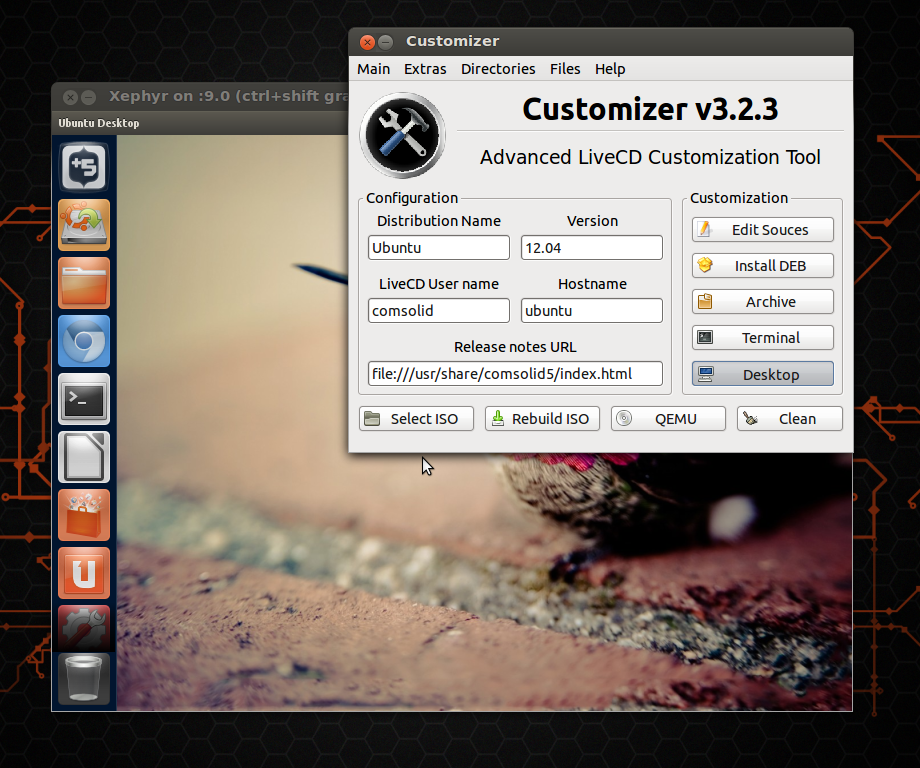
\includegraphics[scale=0.25]{img/customizer.png}
	\caption{Customizer}
\end{figure}

\end{frame}


\begin{frame}\frametitle{Ferramentas de customização}\framesubtitle{Customização, por onde começar?}

Outra ferramenta importante para realizar testes com sua customização é um ambiente de virtualização.

\medskip

Virtualizar significa a grosso modo, rodar um sistema operacional dentro de outro.

\medskip

Uma ótima opção é o VMware Player - \url{http://www.vmware.com/products/player}.

\end{frame}

\begin{frame}\frametitle{Ferramentas de customização}\framesubtitle{Customização, por onde começar?}

Para a customização do Ubuntu 12.04 é necessário conhecer o aplicativo \texttt{gsettings}.

\begin{block}{Exemplo de uso}
\texttt{\$ gsettings get foo bar}
\end{block}

\medskip

O \texttt{gsettings} trabalha com \texttt{schemas}, que são um conjunto de regras que regem um programa,
ou ambiente. Para listar todos os \texttt{schemas} faça:

\begin{block}{Listar schemas}
\texttt{\$ gsettings list-schemas | less}
\end{block}

\end{frame}

\begin{frame}\frametitle{Ferramentas de customização}\framesubtitle{Customização, por onde começar?}

Após achar o \texttt{schema} desejado precisamos listar as \texttt{keys}. Para isso faça:

\begin{block}{Listar keys}
\texttt{\$ gsettings list-keys org.gnome.desktop.interface | less}
\end{block}

\medskip

Podemos agora listar o valor de cada \texttt{key} individualmente usando o comando:

\begin{block}{Listar valor}
\texttt{\$ gsettings get org.gnome.desktop.interface icon-theme}
\end{block}

\end{frame}

\begin{frame}\frametitle{Ferramentas de customização}\framesubtitle{Customização, por onde começar?}

Para modificar o valor de uma \texttt{key} utilizamos o comando:

\begin{block}{Listar valor}
\texttt{\$ gsettings set org.gnome.desktop.interface icon-theme 'Faenza-Dark'}
\end{block}

\medskip

Os valores de uma \texttt{key} podem ser:
\begin{description}
	\item[string] \texttt{'foo'}
	\item[boolean] \texttt{true | false}
	\item[integer] \texttt{0-9}
	\item[array] \texttt{['foo', 'bar']}
\end{description}

\end{frame}

\section{Ambiente de trabalho}

\begin{frame}

\slidetitle{Ambiente de trabalho}

\end{frame}


\subsection{Unity}

\begin{frame}

\slidesubtitle{Unity}

\end{frame}

\begin{frame}\frametitle{Unity}\framesubtitle{Ambiente de trabalho}

Caracteriza-se por uma barra lateral contendo o menu principal e atalhos para os aplicativos
mais utilizados.

\medskip

É o ambiente padrão do Ubuntu desde o 11.04, e vem sofrendo atualizações desde então.

\medskip

Veja mais detalhes em \url{http://unity.ubuntu.com/}

\end{frame}

\subsection{GNOME 3}

\begin{frame}

\slidesubtitle{GNOME 3}

\end{frame}

\begin{frame}\frametitle{GNOME 3}\framesubtitle{Ambiente de trabalho}

A ideia é simplificar a interface e a integrar aos aplicativos, tornando mais direta
a comunicação entre os mesmos.

\medskip

Veja mais em \url{http://www.gnome.org/}

\medskip

Possui suporte a extensões (\url{https://extensions.gnome.org/}) e temas.
O projeto encontra-se em constante atualização, melhorando a usabilidade cada vez mais.

\medskip

Veja um trecho do código \url{http://git.gnome.org/browse/gnome-shell/tree/src/main.c}

\end{frame}

\section{Aplicativos}

\begin{frame}

\slidetitle{Aplicativos}

\end{frame}

\subsection{Multimídia}

\begin{frame}

\slidesubtitle{Multimídia}

\end{frame}

\begin{frame}\frametitle{Multimídia}\framesubtitle{Aplicativos}

Para apresentar as ferramentas multimídia, vamos montar um cenário real de como
seria criar um DVD de clipes no Ubuntu COMSOLiD 5.

Ferramentas necessárias:
\begin{itemize}
	\item Editor de Legendas Gaupol
	\item Criador de Vídeo DVD/CD DeVeDe
	\item Reprodutor de Mídias VLC
\end{itemize}

\end{frame}

\begin{frame}\frametitle{Multimídia}

\begin{columns}

	\begin{column}{4cm}
		% gaupol
		\begin{figure}
			
\includegraphics[scale=0.14]{img/gaupol.png}
			\caption{Gaupol - Editor de Legendas}
		\end{figure}
		
		% devede
		\begin{figure}
			
\includegraphics[scale=0.8]{img/devede.png}
			\caption{DeVeDe - Criador de DVD}
		\end{figure}
	\end{column}

	\begin{column}{4cm}
		% vlc
		\begin{figure}
			
\includegraphics[scale=1.0]{img/vlc.png} 
			\caption{VLC - Reprodutor de Mídias}
		\end{figure}
	\end{column}
	
\end{columns}

\end{frame}

\begin{frame}\frametitle{Take The Time}\framesubtitle{Dream Theater - Images And Words [1992]}

\begin{quote}
"... I need a new {\Large voice}, a new {\Large law}, a {\LARGE new way}\\
Take the time, reevaluate\\
It's time to {\LARGE pick up the pieces},\\
go back to {\large square one}\\
I think it's {\huge time for a change} ..."
\end{quote}

% tradução
\begin{quote}
"... Eu preciso de uma nova voz, uma nova lei, um novo caminho\\
Aproveite o tempo, reavalie\\
É hora de apanhar os pedaços,\\
Voltar ao começo\\
Eu acho que é hora de uma mudança ..."
\end{quote}

\end{frame}

\begin{frame}\frametitle{Multimídia}
Continuando a saga da seção Multimídia, vamos a outro cenário: Extrair e converter
arquivos de um CD de áudio para outros formatos.

Ferramentas utilizadas:
\begin{itemize}
	\item Extrator de CDs de áudio SoundJuicer
	\item Conversor de Som SoundConverter
	\item Ferramenta para Etiquetar Áudio AudioTagTool
\end{itemize}

\end{frame}

\begin{frame}\frametitle{Multimídia}

\begin{columns}

	\begin{column}{4cm}
		% soundjuicer
		\begin{figure}
			
\includegraphics[scale=0.7]{img/soundjuicer.png}
			\caption{Sound Juicer - Extrator de CDs de áudio}
		\end{figure}
		
		% soundconverter
		\begin{figure}
			
\includegraphics[scale=0.7]{img/soundconverter.png}
			\caption{SoundConverter - Conversor de áudio}
		\end{figure}
	\end{column}

	\begin{column}{4cm}
		% audiotagtool
		\begin{figure}
			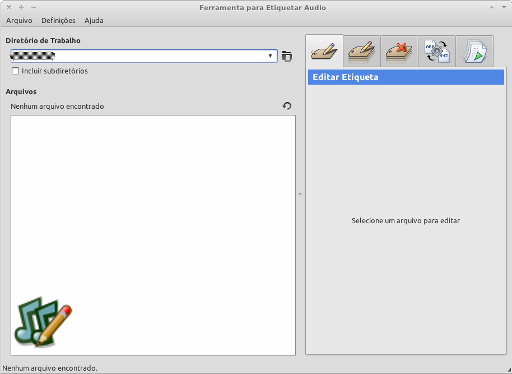
\includegraphics[scale=0.2]{img/audiotagtool.png} 
			\caption{AudioTagTool - Ferramenta para etiquetar áudio}
		\end{figure}
	\end{column}
	
\end{columns}

\end{frame}

\subsection{Escritório}

\begin{frame}

\slidesubtitle{Escritório}

\end{frame}

\begin{frame}\frametitle{LibreOffice}\framesubtitle{Escritório}

\begin{figure}

\includegraphics[scale=0.4]{img/libreoffice.png}
\caption{LibreOffice - App. de Escritório}
\end{figure}

O Ubuntu COMSOLiD 5 já vem com uma versão do LibreOffice atual e completa.
O LibreOffice conta com as seguintes ferramentas:
\begin{itemize}
	\item Writer (Editor de Texto)
	\item Calc (Editor de Planilhas)
	\item Impress (Editor de Slides)
	\item Draw (Editor de Imagens/Desenhos)
	\item Base (Banco de Dados)
	\item Math (Editor de Fórmulas Matemáticas)
	\item e um Administrador de Impressoras.
\end{itemize}

\end{frame}

\subsection{Jogos}

\begin{frame}

\slidesubtitle{Jogos}

\end{frame}

\begin{frame}\frametitle{Jogos}

No Ubuntu COMSOLiD 5 os seguintes jogos podem ser encontrados:
\begin{itemize}
	\item Urban Terror 4.2 HD (Tiro em Primeira Pessoa)
	\item Frogatto (jogo estilo saltar e correr)
	\item ZSNES (Emulador Super Nintendo)
	\item Super Tux Kart (Corrida com Personagens Linux)
	\item PCSX (Emulador PlayStation One)
	\item Mupen64plus (Emulador Nintendo 64)
\end{itemize}

\end{frame}

\begin{frame}\frametitle{ScreenShots}

\begin{columns}
	\begin{column}{4cm}
	% ZSNES
	\begin{figure}
		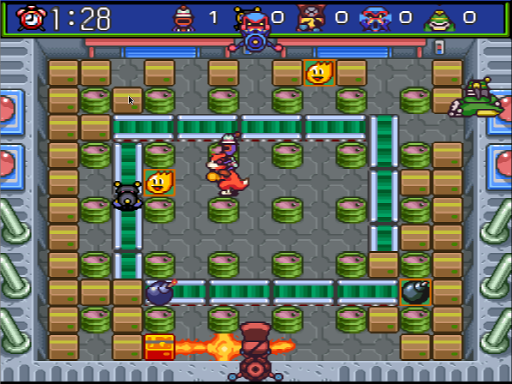
\includegraphics[scale=0.18]{img/zsnes.png}
		\caption{ZSNES}
	\end{figure}
	
	% Open Arena
	\begin{figure}
		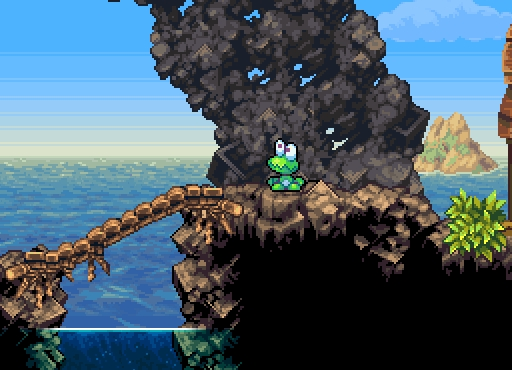
\includegraphics[scale=0.18]{img/frogatto.jpg}
		\caption{Frogatto}
	\end{figure}
	\end{column}
	
	\begin{column}{4cm}
	% Urban Terror
	\begin{figure}
		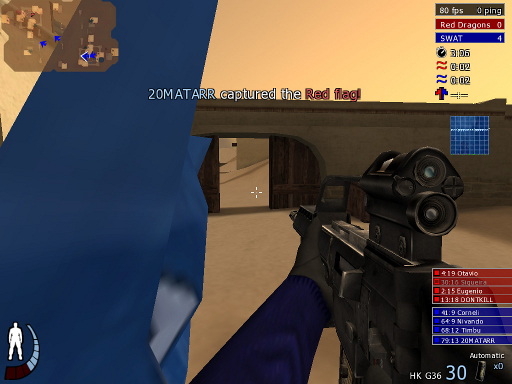
\includegraphics[scale=0.18]{img/urbanterror.jpg}
		\caption{Urban Terror}
	\end{figure}
	
	% STK
	\begin{figure}
		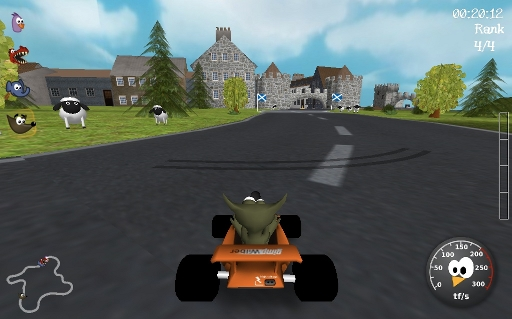
\includegraphics[scale=0.18]{img/stk.jpg}
		\caption{Super Tux Kart}
	\end{figure}
	\end{column}
\end{columns}

\end{frame}

\begin{frame}\frametitle{Onde encontrar esse material?}

\begin{center}
Você pode baixar essa palestra e ainda outras em:

\bigskip

\large{\url{http://www.mad3linux.org/p/downloads.html}}
\end{center}

\end{frame}
